\documentclass[a4paper,twoside,11pt, fleqn]{article}
\usepackage{a4wide,graphicx,fancyhdr,amsmath,amssymb}
\usepackage{listings}
\usepackage{color}
\usepackage{dirtree}
\usepackage{subcaption}

%matlab 
\usepackage[]{mcode}

%----------------------- Macros and Definitions --------------------------

\setlength\headheight{20pt}
\addtolength\topmargin{-10pt}
\addtolength\footskip{20pt}

\newcommand{\N}{\mathbb{N}}
\newcommand{\ch}{\mathcal{CH}}

\newcommand{\solution}[1]{\noindent{\bf Solution to Exercise #1:}}

\fancypagestyle{plain}{%
\fancyhf{}
\fancyhead[LO,RE]{\sffamily\bfseries\large technische universiteit eindhoven}
\fancyhead[RO,LE]{\sffamily\bfseries\large 2IN35 VLSI}
\fancyfoot[LO,RE]{\sffamily\bfseries\large department of mathematics and computer science}
\fancyfoot[RO,LE]{\sffamily\bfseries\thepage}
\renewcommand{\headrulewidth}{0pt}
\renewcommand{\footrulewidth}{0pt}
}

\pagestyle{fancy}
\fancyhf{}
\fancyhead[RO,LE]{\sffamily\bfseries\large technische universiteit eindhoven}
\fancyhead[LO,RE]{\sffamily\bfseries\large 2IN35 VLSI}
\fancyfoot[LO,RE]{\sffamily\bfseries\large department of mathematics and computer science}
\fancyfoot[RO,LE]{\sffamily\bfseries\thepage}
\renewcommand{\headrulewidth}{1pt}
\renewcommand{\footrulewidth}{0pt}

\def\addsquare#1{\tikz\node[draw]{#1};} 

%-------------------------------- Title ----------------------------------

\title{\vspace{-\baselineskip}\sffamily\bfseries Assignment 4}
\author{
	Rick Veens \qquad Studentno: 0912292\\
	\texttt{r.veens@student.tue.nl}
	\and
	Barry de Bruin \qquad Studentno: 0919605\\
	\texttt{e.d.bruin@student.tue.nl}
	\and
	\texttt{Group 7}
}

\date{\today}

\setlength\parindent{0pt}

%--------------------------------- Text ----------------------------------

\begin{document}
\maketitle
\newpage

\tableofcontents

\newpage

\section{Requirements}
\subsection{Analysis of requirements}
\section{System architecture}
The system is implemented in two modules: $filter.v$ and $bram\_mod.v$. $bram\_mod.v$ is but a wrapper around the initialization of a block ram.
The $filter.v$ module contains four block ram modules that store the input samples. Each clock the top values of the block ram's are used to compute a tap. 

This tap is stored in a \textit{Stream delay buffer} that is used to delay an entire stream.
\begin{figure}[h]
	\centering
	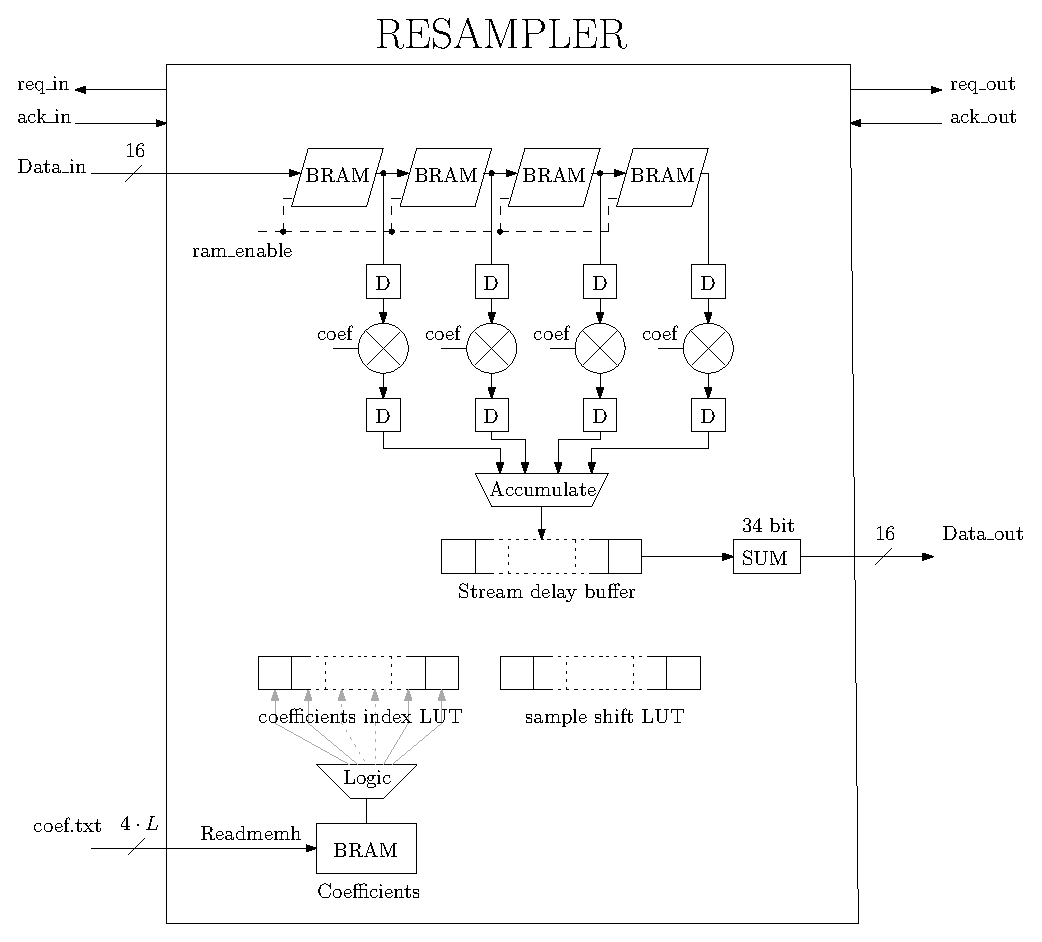
\includegraphics[scale = 1.0]{Images/5_blockdiagram.eps}
    \caption{Abstract functionality of filter.v of the multiple-stream sample rate converter}
    \label{fig:flow}
\end{figure}

\section{Design choices}
\section{Functional correctness}
\section{Resource usage}
\section{System throughput and latency}
\section{Offline project results}
\begin{figure}[h]
	\centering
	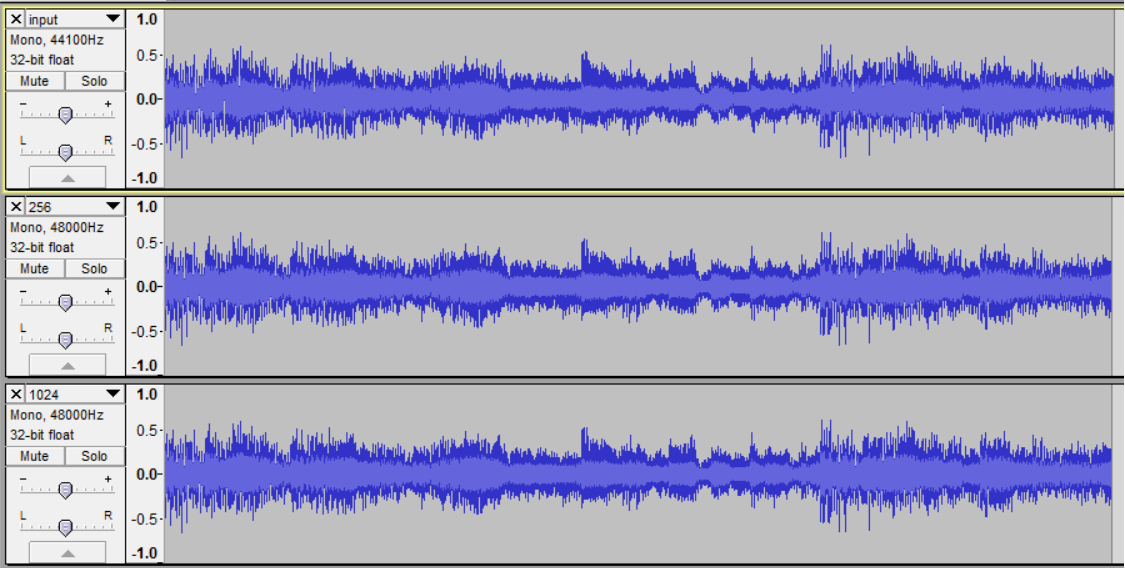
\includegraphics[scale = 0.6]{Images/output_offline.png}
    \caption{Input, and output of 256 and 1024 offline after running on the board.}
    \label{fig:flow}
\end{figure}

\begin{figure}[h]
	\begin{subfigure}[b]{0.5\textwidth}	
		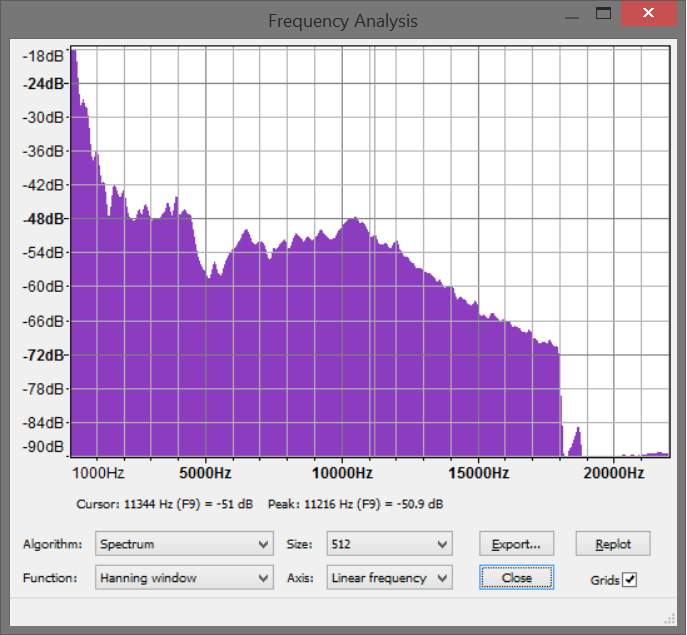
\includegraphics[scale=0.5]{Images/spectrum_input.png}
		\caption{Input}
	\end{subfigure}
	\begin{subfigure}[b]{0.6\textwidth}	
		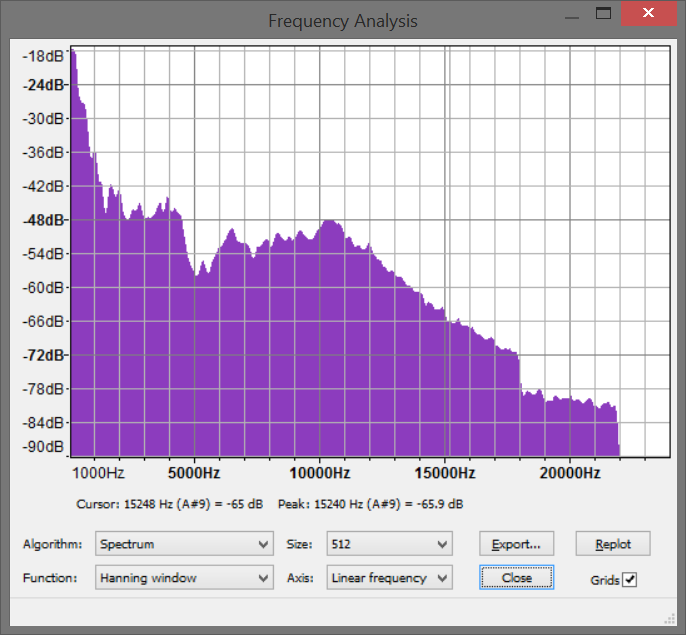
\includegraphics[scale=0.5]{Images/spectrum_offline_256.png}
		\caption{Output of offline-256}
	\end{subfigure}
	\begin{subfigure}[b]{0.6\textwidth}	
		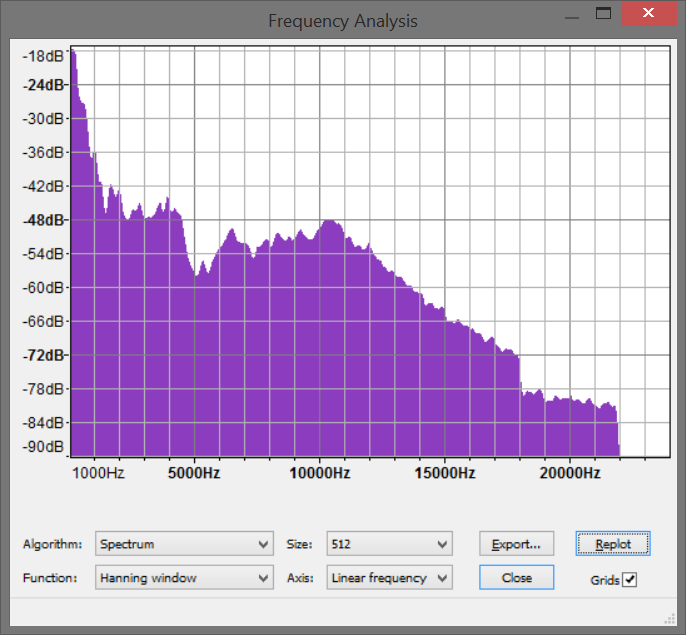
\includegraphics[scale=0.5]{Images/spectrum_offline_1024.png}
		\caption{Output of offline-1024}
	\end{subfigure}
	
    \caption{Comparison of the input spectrum and output spectrums.}
\end{figure}

\newpage

\section{Appendix A: Matlab coefficients script}
\begin{lstlisting}
% Put this in a file named coef_generate_matlab.m, then call it 
% while you are in the file directory. It will write the coefficients
% to the coef.txt file and also return them.

function [y] = coef_generate_matlab(L)
        % make sure that coefficients sum to 1
        y = coef_gen(L);
        y = y/sum(y);

        % quantize and round to nearest integer
        y = y * 160;
        y = round(y*(2^15)); 
             
        % convert to signed int filter coeff
        y = int16(y);
        y = hex(fi(y, 1, 16, 0)); %1 stands for signed, 16 bit out
        
        dlmwrite('coef.txt',y,''); %create file, with no delimiter ''      
end

function [y] = coef_gen(L)
    % generate 4*L coefficients and start at 0 instead of 1 *stupid matlab*
    for n = 1:4*L
            y(n) = lanczos2(((n-1)/L) -2);
    end
end

function y = lanczos2(t)
    if(t <= -2 || t >= 2)
        y = 0;
    else
        y = sinc(t).*sinc(t/2);
    end
end
\end{lstlisting}

Figure~\ref{fig:frq} shows the frequency response of the FIR filter that is generated with help of the matlab code from appendix A.

\begin{figure}[h]
	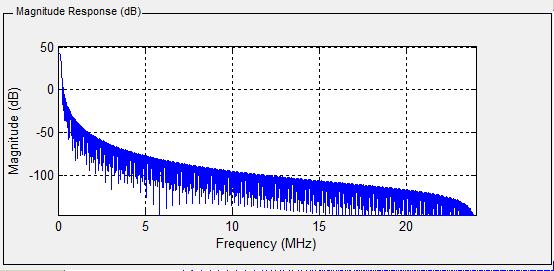
\includegraphics[scale=0.67]{Images/frequencyplot}
    \caption{Interpolation filter frequency domain (Matlab)}
    \label{fig:frq}
\end{figure}

\newpage
\section{Appendix B: Verilog Code}
File: filter.v.
\begin{lstlisting}[language=Verilog]
`timescale 1ns / 1ps

module filter
       #(parameter DWIDTH = 16,
         parameter DDWIDTH = 2*DWIDTH,
         parameter L = 160,
         parameter L_LOG = 8,
         parameter M = 147,
         parameter M_LOG = 8,
         parameter CWIDTH = 4*L,
         parameter NR_STREAMS = 16,
         parameter NR_STREAMS_LOG = 4)
       (input clk,
        input rst,
        output req_in,
        input ack_in,
        input [0:DWIDTH-1] data_in,
        output req_out,
        input ack_out,
        output [0:DWIDTH-1] data_out);

// Output request register
reg req_out_buf;
assign req_out = req_out_buf;

// Input request register
reg req_in_buf;
assign req_in = req_in_buf;

// Accumulator (assigned to output directly)
reg signed [0:DWIDTH-1] sum;
assign data_out = sum;

// RAM wires and registers
reg ram_enable_buf;
wire ram_enable;
assign ram_enable = ram_enable_buf;

reg [0:NR_STREAMS_LOG-1] ram_address_ptr;
wire [0:NR_STREAMS_LOG-1] ram_address;
assign ram_address = ram_address_ptr;

wire [0:DWIDTH-1] ram_data_out[0:3];
reg signed [0:DWIDTH-1] ram_data_out_buf[0:3];

// input buffer
reg signed [0:DWIDTH-1] data_in_buf;
wire [0:DWIDTH-1] data_in_wire;
assign data_in_wire = data_in_buf;

// Instantiate the RAM modules
rom_mod #(DWIDTH, NR_STREAMS_LOG)
        bram_0 (clk, rst, ram_enable, ram_address, data_in_wire, ram_data_out[0]);
rom_mod #(DWIDTH, NR_STREAMS_LOG)
        bram_1 (clk, rst, ram_enable, ram_address, ram_data_out[0], ram_data_out[1]);
rom_mod #(DWIDTH, NR_STREAMS_LOG)
        bram_2 (clk, rst, ram_enable, ram_address, ram_data_out[1], ram_data_out[2]);
rom_mod #(DWIDTH, NR_STREAMS_LOG)
        bram_3 (clk, rst, ram_enable, ram_address, ram_data_out[2], ram_data_out[3]);

// pipeline stage
reg signed [0:DDWIDTH-1] pl_mul_to_acc_buf[0:3];

// intialize buffers
reg shift_enable;
integer sample_index, buf_ptr;
reg [0:L-1]lookup_shift; //'1' means shift, '0' means no shift
reg signed [0:DWIDTH-1] coef [0:CWIDTH-1], lookup_coefIdx[0:L-1][0:3], coef_preproc[0:3];

reg signed [0:DDWIDTH+1] stream_delay_buf[0:NR_STREAMS-1];


integer i, j;
initial begin
    for(i = 0; i < 4; i = i + 1) begin
        pl_mul_to_acc_buf[i] <= 0;
        ram_data_out_buf[i] <= 0;
    end

    // define shift LUT
    for(i=0;i<L;i=i+1) begin
        if(i*M/L == (i+1)*M/L)
            lookup_shift[i] = 0; //do not shift yet
        else
            lookup_shift[i] = 1; //shift
    end

    // define coef LUT
    for (i = 0; i < L; i = i + 1) begin
        for(j = 0; j < 4; j = j + 1) begin
            lookup_coefIdx[i][j] = j*L + i*M%L;
        end
    end

    for (i = 0; i < NR_STREAMS; i = i + 1) begin
        stream_delay_buf[i] <= 0;
    end

    // import coefficients
    $readmemh("coef.txt", coef, 0, CWIDTH -1);
end

always @(posedge clk) begin
    // Reset => initialize
    if (rst) begin
        req_in_buf <= 0;
        req_out_buf <= 0;
        sum <= 0;
        sample_index <=0;
        buf_ptr <= 0;
        shift_enable <= 0;
        data_in_buf <= 0;
        ram_enable_buf <= 1;
        ram_address_ptr <= 0;
    end
    // !Reset => run
    else begin

        // Read handshake complete
        if (req_in && ack_in) begin
            // shift data in.
            data_in_buf <= data_in;
            ram_enable_buf <= 1;

            req_in_buf <= 0;
        end

        // data shifted in ram
        if (ram_enable_buf== 1) begin
            ram_enable_buf <= 0;
        end

        // Write handshake complete
        if (req_out && ack_out) begin

            // See if we have to shift next stream of samples
            if(ram_address_ptr == NR_STREAMS-1) begin
                shift_enable <= lookup_shift[sample_index];
                sample_index <= (sample_index + 1) % L;
            end

            // if so, ask for new input data
            if(shift_enable == 1) begin
                req_in_buf <= 1;
            end
            else begin
                // do NOT ask for new input data, re-use buffered data (stream_delay_buf)
            end
            req_out_buf <= 0;
        end

        // Processing state
        if (!req_in && !ack_in && !req_out && !ack_out && ram_enable_buf == 0) begin

            //retrieve samples
            ram_data_out_buf[0] <= ram_data_out[0];
            ram_data_out_buf[1] <= ram_data_out[1];
            ram_data_out_buf[2] <= ram_data_out[2];
            ram_data_out_buf[3] <= ram_data_out[3];

            //multiply with coefficients
            pl_mul_to_acc_buf[0] <= ram_data_out_buf[0]*coef_preproc[0];
            pl_mul_to_acc_buf[1] <= ram_data_out_buf[1]*coef_preproc[1];
            pl_mul_to_acc_buf[2] <= ram_data_out_buf[2]*coef_preproc[2];
            pl_mul_to_acc_buf[3] <= ram_data_out_buf[3]*coef_preproc[3];

            //accumulate and put into delay buffer
            stream_delay_buf[buf_ptr]	<= 	pl_mul_to_acc_buf[0] +
                            pl_mul_to_acc_buf[1] +
                            pl_mul_to_acc_buf[2] +
                            pl_mul_to_acc_buf[3];

            // increment pointers
            ram_address_ptr <= (ram_address_ptr + 1) % NR_STREAMS;
            buf_ptr <= (buf_ptr + 1)%((NR_STREAMS));

            // output data (+2 offset is the delay of the pipeline)
            sum <= stream_delay_buf[(buf_ptr+2)%NR_STREAMS][3:DWIDTH+2];

            // preprocess next coefficients
            coef_preproc[0] <= coef[lookup_coefIdx[sample_index][0]];
            coef_preproc[1] <= coef[lookup_coefIdx[sample_index][1]];
            coef_preproc[2] <= coef[lookup_coefIdx[sample_index][2]];
            coef_preproc[3] <= coef[lookup_coefIdx[sample_index][3]];

            // request output
            req_out_buf <= 1;
        end

    end
end

endmodule
\end{lstlisting}

\newpage

File: bram$\_$mod.v.
\begin{lstlisting}[language=Verilog]
`timescale 1ns / 1ps
module rom_mod
       #(parameter RAM_WIDTH = 16,
         parameter RAM_ADDR_BITS = 10 )(
           input clk,
           input rst,
           input enable,
           input [0:RAM_ADDR_BITS-1] ram_address,
           input [0:RAM_WIDTH-1] in_data,
           output [0:RAM_WIDTH-1] out_data);

(* RAM_STYLE="block" *)
reg [RAM_WIDTH-1:0] bram [(2**RAM_ADDR_BITS)-1:0];
wire [RAM_ADDR_BITS-1:0] ram_address_ptr;

// output buffer
//reg [0:RAM_WIDTH-1] data_out_buf;
assign out_data = bram[ram_address_ptr];

// reverse all address wires
generate
    genvar j;
for(j=0;j<RAM_ADDR_BITS;j=j+1) begin: reverse
    assign ram_address_ptr[j] = ram_address[j];
end
endgenerate

    integer i;
initial begin
    for(i=0;i<2**RAM_ADDR_BITS-1;i=i+1)
        bram[i] <= 0;
end

always @(posedge clk) begin
    if(rst) begin
        //data_out_buf <= 0;
    end
    else begin
        if (enable) begin
            bram[ram_address_ptr] <= in_data;
        end
        //data_out_buf <= bram[ram_rd_address];
    end
end
endmodule
\end{lstlisting}

\end{document}
